\section{Execution Time, Energy and Carbon of the Corrected Models}\label{sec:energy}
This separate stage reads the equal-evaluation caches and measures execution of their selected models. It does not alter $C_\rho$, either declared weight or the $\tau$-rule. Historical energy measurements are not included.
\subsection{Reconstruction and execution implementations}
The 450 selected records comprise SO, MO-lex and Green under $\rho=1$, and MO-lex and Green under $\rho_K$, across three examples and 30 seeds. Four failed validations remain missing; 446 models were rebuilt, re-estimated and checked against their saved costs and validation errors. The primary canonical simulator evaluates the duplicate-free polynomial in straight-line Python with exactly $a$ additions and $b$ multiplications per sample. The secondary NumPy simulator evaluates every gene with corrected delays; it is not the unmodified package predictor. The two implementations agree within the declared reconstruction tolerances.
\subsection{Timing, power integration and carbon conversion}
Each model's timing is the median of five repeated-simulation batches lasting at least 50~ms. Power was measured in a separate mains-powered session on an Apple M2 with Python 3.13.9, using CPU, GPU and neural-engine power from \texttt{powermetrics} at 100~ms intervals. Ten rounds each visit 30 groups in a fixed seeded random order, with complete cycles over the valid models of each group for at least 10~s. Eleven idle blocks bracket the rounds, giving 311 blocks in total. Every block has valid power samples.

Net energy per simulation is
\begin{equation}
E_{\mathrm{sim}}=\frac{E_{\mathrm{block}}-\widetilde P_{\mathrm{idle}}t_{\mathrm{block}}}{n_{\mathrm{sim}}},\label{eq:esim}
\end{equation}
where the baseline is the median power across all idle blocks. Idle block means range from \CorrectedIdleMin{} to \CorrectedIdleMax{}~W. Replacing the baseline by the mean of the two idle blocks bracketing each round leaves all Holm-significance decisions unchanged in the sensitivity analysis. CodeCarbon supplies only the Irish grid intensity, \CorrectedCI{}~gCO$_2$e/kWh~\cite{codecarbon}; emissions are $E_{\mathrm{sim}}I_{\mathrm{grid}}$ after conversion to kWh. CodeCarbon does not track energy inside the measurement blocks and neither power nor carbon intensity establishes $\rho$.

Energy ratios to SO are formed within each round. Green is compared with SO, MO-lex and Green-K using two-sided Mann--Whitney tests over rounds, with Holm correction across the 18 example--simulator--comparator tests and $A_{12}$. These are within-session comparisons, not independent hardware sessions.
\subsection{Time-based assessment of the fixed weights}
For \CorrectedNStructures{} distinct canonical structures, the fit $t=t_0+t_+a+t_\times b$ gives $t_+=\CorrectedTadd$~ns, $t_\times=\CorrectedTmul$~ns and $R^2=\CorrectedRtwoOps$. The ratio $t_\times/t_+=\CorrectedMulAdd$ is close to one for this Python implementation. The operation-count fit has $R^2=\CorrectedRtwoOne$, compared with \CorrectedRtwoK{} for the Karatsuba-weighted cost. These measurements support the scale of the already fixed unit weight; they do not retune the completed searches. The coefficients include interpreter overhead, are fitted to search-selected structures and do not measure instruction-level costs. The separate C microbenchmark is a diagnostic of another execution implementation.
\begin{figure}[!htbp]\centering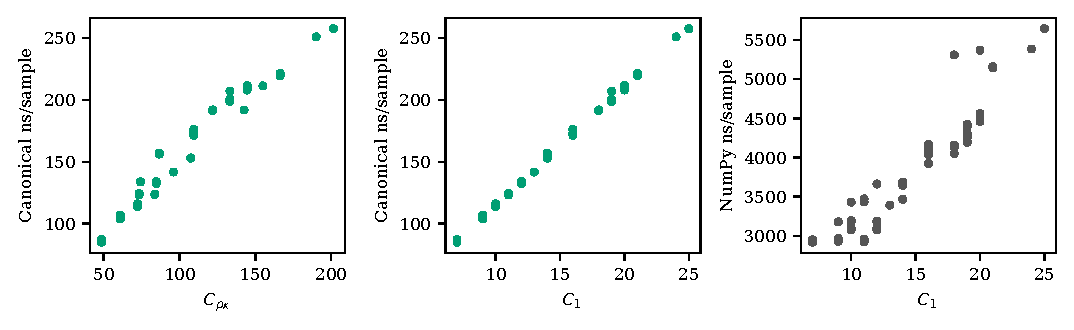
\includegraphics[width=\textwidth]{figures/fig_exec_time.pdf}\caption{Corrected-model execution time per sample: canonical simulation against $C_{\rho_K}$ and $C_1$, and corrected all-gene NumPy simulation against $C_1$. Both search weights are represented.}\label{fig:exectime}\end{figure}
\subsection{Energy results and their limits}
\begin{table}[!htbp]
\centering
\caption{Execution of the corrected selected models: median time, net energy and estimated carbon per simulation over ten measurement rounds. Canonical execution evaluates distinct monomials; all-gene NumPy execution uses corrected delays. Suffix K denotes searches under $\rho_K$.}
\label{tab:corrected_energy}
\setlength{\tabcolsep}{3pt}
\begin{tabular}{llrrrrrr}
\toprule
 & & \multicolumn{3}{c}{Canonical polynomial} & \multicolumn{3}{c}{All-gene NumPy} \\
\cmidrule(lr){3-5}\cmidrule(lr){6-8}
Ex. & Method & Time ($\mu$s) & Energy ($\mu$J) & CO$_2$e ($\mu$g) & Time ($\mu$s) & Energy ($\mu$J) & CO$_2$e ($\mu$g) \\
\midrule
E1 & SO & 9.91 & 65.4 & 0.00528 & 313 & 2.11e+03 & 0.17 \\
E1 & MO-lex & 7.78 & 51.6 & 0.00417 & 329 & 2.31e+03 & 0.186 \\
E1 & Green & 7.79 & 52.2 & 0.00422 & 337 & 2.37e+03 & 0.192 \\
E1 & MO-lex-K & 7.82 & 52.5 & 0.00424 & 334 & 2.32e+03 & 0.187 \\
E1 & Green-K & 7.78 & 51.1 & 0.00413 & 330 & 2.35e+03 & 0.19 \\
\midrule
E2 & SO & 11.7 & 76.7 & 0.0062 & 338 & 2.34e+03 & 0.189 \\
E2 & MO-lex & 9.49 & 65.7 & 0.0053 & 328 & 2.24e+03 & 0.181 \\
E2 & Green & 7.66 & 51.2 & 0.00414 & 324 & 2.23e+03 & 0.18 \\
E2 & MO-lex-K & 9.44 & 62.7 & 0.00507 & 326 & 2.23e+03 & 0.18 \\
E2 & Green-K & 7.65 & 50.4 & 0.00407 & 321 & 2.25e+03 & 0.182 \\
\midrule
E3 & SO & 38.4 & 251 & 0.0203 & 848 & 5.8e+03 & 0.469 \\
E3 & MO-lex & 35.3 & 232 & 0.0188 & 832 & 5.55e+03 & 0.448 \\
E3 & Green & 33.6 & 228 & 0.0184 & 789 & 5.26e+03 & 0.425 \\
E3 & MO-lex-K & 35.4 & 233 & 0.0188 & 830 & 5.6e+03 & 0.452 \\
E3 & Green-K & 32.9 & 219 & 0.0177 & 783 & 5.38e+03 & 0.434 \\
\bottomrule
\end{tabular}
\end{table}

Table~\ref{tab:corrected_energy} gives absolute time, energy and carbon estimates, while Fig.~\ref{fig:energy} compares energy relative to SO within each round. In that figure, values below one indicate savings and values above one an increase; the bars describe variation over rounds in this session. For canonical execution, median per-round Green/SO energy ratios are \CorrectedEBEnergyRatio, \CorrectedECEnergyRatio{} and \CorrectedEDEnergyRatio{} on E1--E3. The corresponding reductions are \CorrectedEBCanReduction\%, \CorrectedECCanReduction\% and \CorrectedEDCanReduction\%. Reductions are significant against SO on E1 and E2 (Holm-adjusted $p=\CorrectedEBCanP$ and $p=\CorrectedECCanP$), whereas the E3 difference is not significant ($p=\CorrectedEDCanP$). Green differs significantly from MO-lex in canonical energy only on E2, and not from Green-K on any example after Holm correction.

The secondary implementation changes the outcome: on E1 Green uses \CorrectedEBNumpyIncrease\% more energy than SO ($p=\CorrectedEBNumpyP$). E2 shows no significant difference against SO ($p=\CorrectedECNumpyP$); on E3 Green uses \CorrectedEDNumpyReduction\% less energy ($p=\CorrectedEDNumpyP$), and also differs from MO-lex. Arithmetic savings of the canonical polynomial therefore do not guarantee savings when all genes are executed through NumPy.
\begin{figure}[!htbp]\centering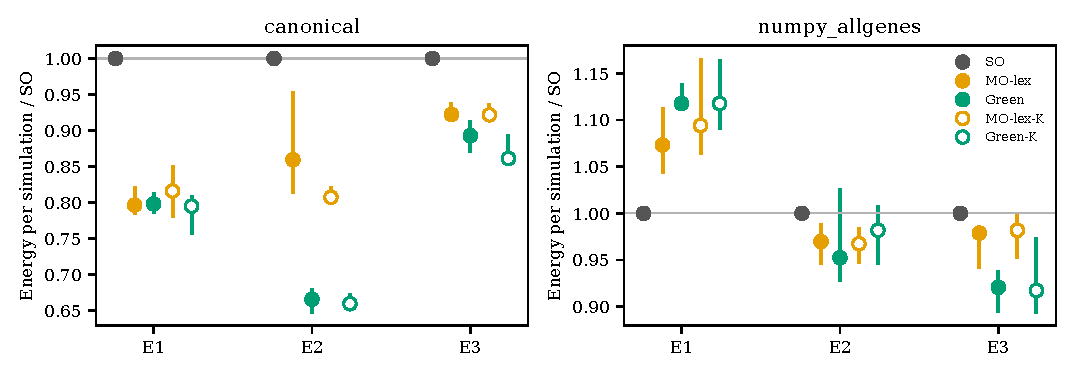
\includegraphics[width=\textwidth]{figures/fig_energy.pdf}\caption{Corrected selected-model energy relative to SO within each of ten rounds: medians and interquartile ranges. Open markers denote the Karatsuba-weighted searches; the secondary simulator uses corrected delays.}\label{fig:energy}\end{figure}
These findings concern interpreted execution on one laptop system-on-chip in one session. They do not establish embedded-hardware performance or a universal multiplication weight. E3 selected models generalise poorly under the unchanged identification-only rule, so energy reductions cannot be presented as savings at preserved validation accuracy. Carbon values are energy-derived estimates using one grid-intensity factor, not directly measured emissions.
\FloatBarrier
